%%%%%%%%%%%%%%%%%%%%%%%%%%%%%%%%%%%%%%%%%%%%%%%%%%%%%%%%%%%%%%%%%%%%%%%%%%%%%%%%
\chapter{ПРОЕКТИРОВАНИЕ АРХИТЕКТУРЫ МОДУЛЯ}
%%%%%%%%%%%%%%%%%%%%%%%%%%%%%%%%%%%%%%%%%%%%%%%%%%%%%%%%%%%%%%%%%%%%%%%%%%%%%%%%

На рисунке \ref{image:architecture} изображена архитектура модуля. Опишем каждую его часть.

\begin{figure}[h!]
\center{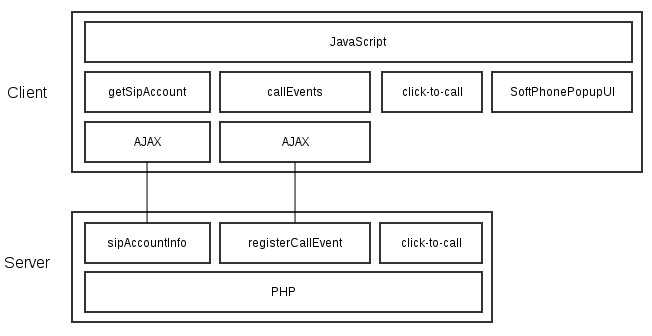
\includegraphics[width=0.8\linewidth]{architecture}}
\caption{Архитектура модуля}
\label{image:architecture}
\end{figure}

Основой модуля является его ядро softPhoneJS. Ядро обеспечивает взаимодействие с sipML5 и переключает состояние звонка. При переключении состояния информация передаётся в модуль CallEvents, который является зависимым от web-приложения, и далее отправляет информацию на сервер, для регистрации звонка.

Только перед тем как звонить, необходимо получить из CRM-системы данные о SIP-аккаунте. За это отвечает модуль getSipAccount.

SoftPhonePopupUI отвечает за графический интерфейс скользящей кнопки и плавающего окна. Так же графический интерфейс реагирует на состояние звонка, например, запрещая пользователю нажимать на кнопку сброса пока звонок ещё не начался.

Click-to-call реализован на сервере, так как он должен добавлять функцию обработчика на html-страницу, получаемую от сервера. Обработчик вызывается при нажатии на номер телефона на странице web-приложения и заполняет поле номера на плавающем окне.
